\mychapter{Image Processing}{Image Processing}{}
\label{chap:imgpros}

\mysection{Introduction}{Introduction}
\label{sec:imgintro}

\mysection{Pinhole Camera Model}{Pinhole Camera Model}
\label{sec:imgpinhole}

The ideal pinhole camera can be described as a plane and an optical center (a.k.a) the pinhole. Light will travel from an object throught the optical center.
And hit the plane at the opposite end of the optical center. The distance between the opitical center and the plane is called the focal length $f$.


\begin{figure}[H]
    \centering
    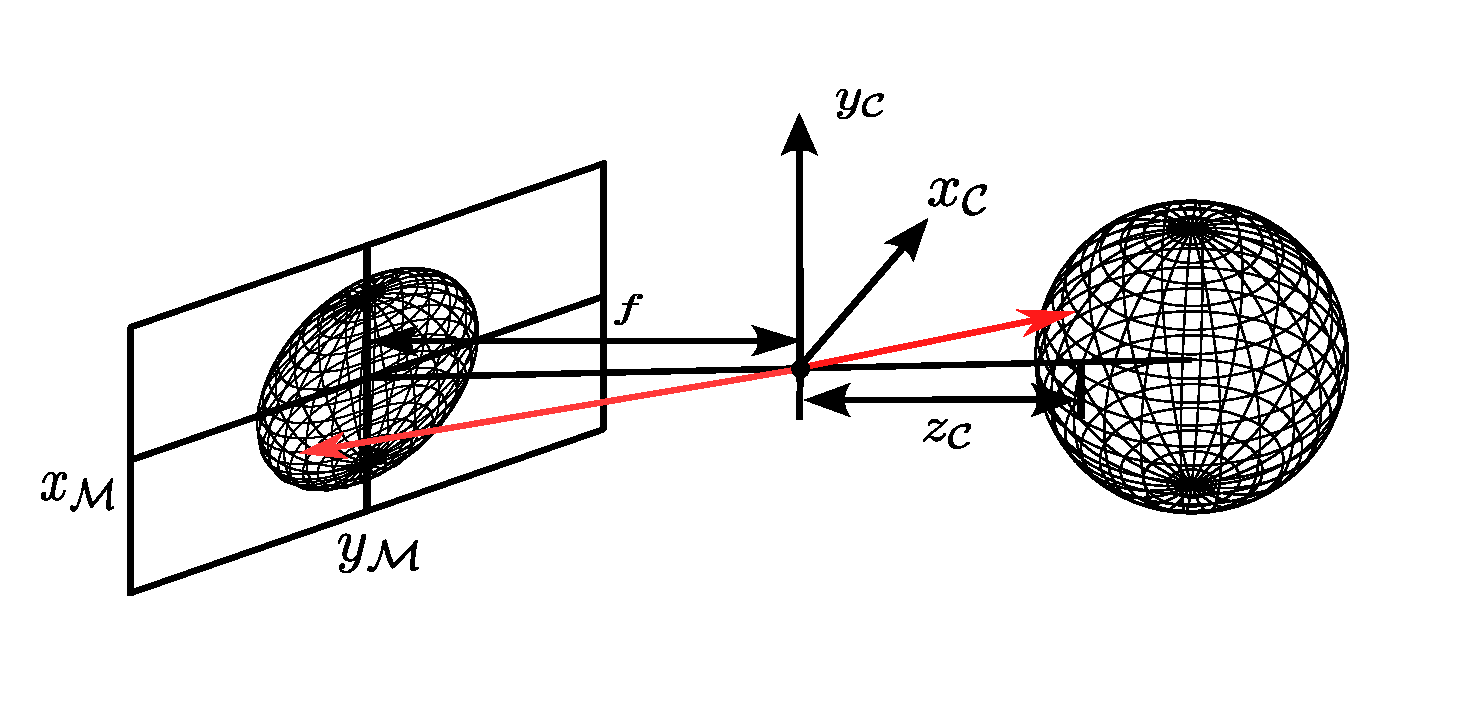
\includegraphics[width=1\linewidth]{figures/imageprocessing/Pinhole.pdf}
    \caption{PinHole Model}
    \label{fig}
\end{figure}


The equation for the pinhole camera model is the following.

\begin{equation}
\begin{bmatrix}
    x_\mathcal{M} \\
    y_\mathcal{M} \\
    1 
\end{bmatrix}
= \frac{-f}{z_\mathcal{C}}
\begin{bmatrix}
    x_\mathcal{C} \\
    y_\mathcal{C} \\
    z_\mathcal{C}
\end{bmatrix}
\end{equation}

As we can see in the figure this also causes the image tp flip.

Also images are measured with the x-axis going from right to left and the y-axis going from top to bottom so one more transformation needs to be done.

\begin{figure}[H]
    \centering
    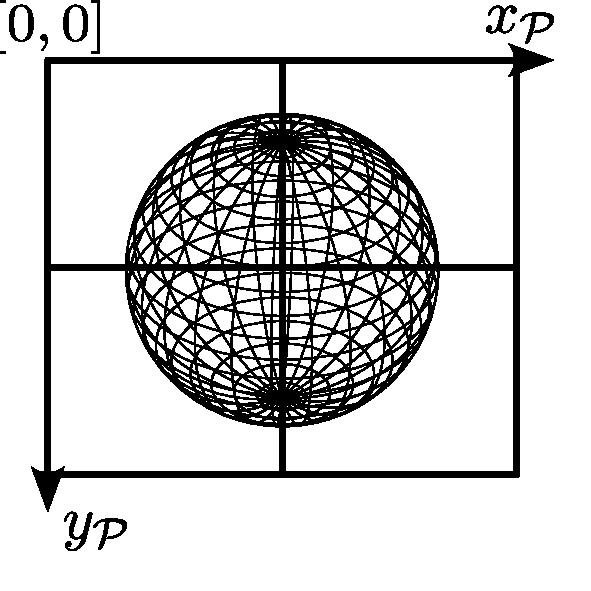
\includegraphics[width=0.5\linewidth]{figures/imageprocessing/ImagePlane.pdf}
    \caption{Image Plane}
    \label{fig4.2}
\end{figure}

\begin{equation}
\begin{bmatrix}
x_\mathcal{P} \\
y_\mathcal{P}
\end{bmatrix}
=
\begin{bmatrix}
    -x_\mathcal{M} + \frac{\text{ImgWidth}}{2} \\
    y_\mathcal{M} + \frac{\text{ImgHeight}}{2}
\end{bmatrix}
\end{equation}


\mysection{Satellite Image Characteristics}{Satellite Image Characteristics}

\mysubsection{Ground Sample Distance}{Ground Sample Distance}
% Mathematical relationship


% Impact on feature detection accuracy
% Trade oofs with altitude and camera parameters


\mysubsection{Imaging Geometry}{Imaging Geometry}

% Nadir vs off-nadir imaging
% Field of view calculations
% Ground coverage estimation
% Geometric distortions

\mysection{Feature Detection and Description}{Feature Detection and Description}

\mysubsection{Classical Feature Detectors}{Classical Feature Detectors}
% SIFT
% SURF
% ORB
% Harris corner detection
% Comparision for satellite application

\mysubsection{Feature Description}{Feature Description}
% Local feature descriptors
% Invariance properties (scale, rotation, illumination)
% Descriptor Matching stratagies
% Robustness to viewpoint changes

% \mysubsection{Feature Quality Assessment}{Feature Quality Assessment}


\mysection{Measurement Extraction}{Measurement Extraction}
\label{sec:imgmesurement}

\mysubsection{Feature-to-Measurement Transformations}{Feature-to-Measurement Transformation}
% Pxiel coordinates to e metric coordinates
% Ray vector computation from image features
% Uncertainty propagration through camera model
% Measurement noise characterisation

\mysubsection{Earth Tracker Algorithm}{Earth Tracker Algorithm}
% Pixel coordinate extraction from features
% Translation to optical center coordinates
% 3D ray vector construction
% Metric scaling using GSD
% Coordinate frame transformations

\mysubsection{Geolocation Process}{Geolocation Process}
% Direct geolocation methods
% Feature correspondence establishment
% Geographic coordinate conversion
% Accuracy validation techniques



